%chap 5
\chapter{شبیه‌سازی و ارزیابی مدل پیشنهادی}
\label{chap5}
\thispagestyle{empty}
\section{مقدمه}
\label{chap5sec1}
در فصل پیشین مدل پیشنهادی در این پژوهش به طور کامل معرفی‌ گردید و با بخش‌ها و روابط موجود در آن کاملا آشنا شدیم. در این فصل رویکرد معرفی‌ شده در این پایان‌‌نامه مورد  ارزیابی و آزمایش قرار می‌‌گیرد و نتایج بدست آمده در آزمایش‌های گوناگون را مورد تحلیل و بررسی‌ قرار می‌‌دهیم. در این فصل ابتدا پیش‌پردازش‌های لازم و مطرح در بحث 
NLP
را که از آن‌ها برای آماده‌سازی پایگاه داده استفاده می‌کنیم شرح داده و سپس پایگاه داده‌ی مورد استفاده در این فصل را معرفی کرده و خصوصیات آن را در سه‌ حالت مختلف بیان می‌‌کنیم، سپس یک معیار معروف به نام سرگشتگی\footnote{Perplexity}
که از آن برای ارزیابی مدل‌های احتمالی‌ مولد استفاده می‌شود و در ادامه از آن برای ارزیابی مدل پیشنهادی استفاده می‌‌کنیم را تعریف می‌‌کنیم. در بخش‌های بعدی آزمایشات انجام شده بر روی پایگاه داد‌ه‌ی معرفی‌ شده را به تفصیل شرح می‌‌دهیم و نتایج بدست آمده را تحلیل می‌‌کنیم.

\section{پیش‌پردازش‌های متنی در پردازش زبان طبیعی}
\label{chap5sec2}
در مباحث مربوط به
NLP
مخصوصاً روش‌ها و رویکردهایی که با داده‌های متنی سر و کار دارند، پیش از اینکه داده‌ها به مدل وارد شوند بر روی آن‌ها پیش‌پردازش‌های تاثیر گذاری انجام می‌‌شود که ما نیز برای آماده‌سازی داده‌ها جهت ورود به مدل این کار را انجام داده و پس از تبدیل داده‌های متنی به شکلی‌ استاندارد آن‌ها را به مدل وارد کردیم. چهار پیش پردازش لازم جهت آماده سازی داده‌های متنی به ترتیب اجرا بر روی پایگاه داده به صورت:
\begin{enumerate}
	\item علامت‌گذاری و حذف کارکترهای بی‌معنی\footnote{Tokenization and Remove Meaningless Characters}
	\item ریشه یابی لغوی\footnote{Stemming}
	\item ریشه یابی نحوی\footnote{Lemmatization}
	\item حذف کلمات توقف\footnote{Remove Stop Words}
\end{enumerate}
می‌ باشند که در ادامه به تعریف آنها می‌‌پردازیم.
\subsection{علامت‌گذاری و حذف کاراکترهای بی‌معنی‌}
\label{chap5sec2sub1}
در این مرحله هر جمله به کلمات تشکیل دهنده‌ی آن شکسته می‌‌شود و سپس تمام کاراکترهای اضافه‌ای ‌که در واژگان زبان وجود نداشته باشند از جمله حذف می‌‌گردند. برای مثال در این مرحله نقطه گذاری‌ها، پرانتزها، کاراکتر‌های خاص مانند
$@,  \star $
و غیره از تمام اسناد در پایگاه داده حذف می‌‌شوند.

\subsection{ریشه یابی لغوی}
\label{chap5sec2sub2}
ریشه یابی‌ لغوی به معنی‌ تبدیل حالت‌های مختلف یک کلمه که در متن وجود دارند به یک صورت واحد و یکتا است. به طور مثال در زبان انگلیسی می‌‌توان به مواردی نظیر حذف
ing
از پایان کلمات یا حذف
's
مالکیت از انتهای اسامی اشاره کرد. برای درک بهتر به مثال زیر توجه کنید که در آن تمام حالت‌های سمت چپ در فرآیند پیش‌پردازش  ریشه یابی  لغوی به حالت سمت راست تبدیل می‌‌شوند.\\
\begin{latin}
	$car, cars, car's, cars' \rightarrow car$
\end{latin}


\subsection{ریشه یابی نحوی}
\label{chap5sec2sub3}
علی‌رغم نتایج یکسان برای ریشه یابی‌ لغوی و نحوی در بسیاری از حالت‌ها، اما تفاوت فراوانی‌ بین این دو پیش‌پردازش وجود دارد. در بحث ریشه یابی‌ نحوی ما به دنبال یافتن ریشه‌ی افعال و کلمات موجود در متن هستیم و بسیاری از کلمات و افعال به شکل مصدری خود بازگردانده می‌‌شوند. ریشه یابی‌ لغوی برای هر کلمه به صورت جداگانه و بدون در نظر گرفتن مفهوم متن انجام می‌‌شود، اما در حالت نحوی با توجه به مفهوم، کلماتی‌ که شکل یکسانی دارند اما معنی آن‌ها متفاوت است به مصدر های مختلفی تبدیل می‌‌شوند. به طور مثال در زبان انگلیسی‌ برای کلمه‌ای‌ مانند
Walking
نتیجه‌ی حاصل از هر دو ریشه یابی‌ نحوی و لغوی کلمه‌ی
Walk
است. اما برای سه‌ فعل کمکی‌ مانند
$am, is, are$
با انجام ریشه یابی‌ لغوی تغییری در آن‌ها اتفاق نمی‌افتد، اما با ریشه یابی  نحوی هر سه‌ کلمه به حالت
be
تغییر شکل می‌‌دهند.\\
\begin{latin}
	``Walking'' $ with \ Stemming \rightarrow$ Walk \quad\quad ``Walking'' $ with \ Lemmatization \rightarrow$ Walk\\


	``Am, Is, Are'' $ with \ Stemming \rightarrow$ Am, Is, Are \quad\quad ``Am, Is, Are'' $ with \ Lemmatization \rightarrow$ be\\
\end{latin}

\subsection{حذف کلمات توقف}
\label{chap5sec2sub4}
در هر زبانی لغات بسیاری هستند که آن‌ها را کلمات عمومی یا کلمات توقف آن زبان تعریف می‌‌کنند. این کلمات به صورت گسترده و فراوان در متن یافت می‌‌شوند و هیچ‌گونه بار اطلاعاتی با خود به همراه ندارند. حذف این کلمات از داده‌های متنی علاوه بر کوچک کردن اندازه داده‌ی ورودی به مدل منجر به بهبود کیفیت نتایج شده و کارایی مدل را افزایش می‌‌دهد. در ادامه چند نمونه از این کلمات برای زبان انگلیسی‌ آورده شده است.\\
\begin{latin}
	me, my, myself, ourselves, can, will, just, ...
\end{latin}



\section{پایگاه داده‌ی بازبینی فیلم}
\label{chap5sec3}
پایگاه داد‌ه‌ی بازبینی فیلم\footnote{Movie Review}
(MR)
 پس از استفاده در کار
Pang
و همکاران
\cite{pang2002thumbs}
تبدیل به یک معیار در بحث مدل‌سازی احساس و همچنین ارزیابی مدل‌های پیشنهاد شده گردیده است
\cite{lin2012weakly}.
نسخه~۲\footnote{Available at http://www.cs.cornell.edu/people/pabo/movie-review-data}
از این پایگاه داده که ما در آزمایش‌های خود از آن استفاده می‌‌کنیم شامل ۱۰۰۰ بازبینی مثبت از فیلم‌های مختلف و ۱۰۰۰ بازبینی منفی‌ می‌‌باشد. این بازبینی‌ها از سایت پایگاه داد‌ه‌ی اینترنتی فیلم\footnote{Internet Movie Database}
(IMDB)
جمع‌آوری شده‌اند. میانگین طول هر بازبینی در این پایگاه داده ۳۰ جمله می‌‌باشد که بر روی آن پیش پردازش معرفی شده در بخش‌های
\ref{chap5sec2sub1}
تا 
\ref{chap5sec2sub2}
 را انجام می‌دهیم  و در ادامه مراحل آن را شرح می‌دهیم.
 
 
 \section{پایکاه داده‌ی 20 گروه خبری}
 \label{chap5sec11}
 پایگاه داده‌ی ۲۰ گروه خبری\footnote{News Groups, Available at http://people.csail.mit.edu/jrennie/20Newsgroups}
(20NG)
 یکی‌ از دیتاست‌های معروف در بحث مدل‌سازی موضوع است. این پایگاه داده شامل ۱۸۷۸۶ سند متنی است که از مخازن گروه‌های خبری
 Usenet
 جمع‌آوری شده‌اند. این مجموعه سند به ۲۰ گروه خبری مختلف تقسیم می‌‌شود که هر کدام از این ۲۰ گروه مربوط به یک موضوع خاص هستند. از مجموع ۱۸۷۸۶ سند موجود در این پایگاه داده، ۱۱۲۸۴ سند برای مجموعه‌ی آموزش و ۷۵۰۲ سند برای مجموعه‌ی تست در نظر گرفته می‌‌شوند. پس از انجام پیش‌پردازش‌های گفته‌ شده در بخش
 \ref{chap5sec2}،
 ۲۰۰۰ کلمه‌ای‌ که بیشترین تکرار را دارند جدا شده و به عنوان لغت‌نامه برای این پایگاه داده در نظر گرفته می‌‌شوند. در بخش‌های بعدی از لغت‌نامه‌ی این پایگاه داده برای ارزیابی‌های بسیاری استفاده می‌کنیم. همچنین در بخش 
 \ref{chap5sec10}
 از این پایگاه داده استفاده و نتایج بدست آمده از بازیایی اطلاعات بر روی آن را گزارش می‌کنیم.
 
 \section{پایگاه داده‌ی احساس چند دامنه}
 \label{chap5sec12}
 پایگاه داده‌‌ی احساس چند دامنه\footnote{Multi Domain Sentiment, Available at http://www.cs.jhu.edu/~mdredze/datasets/sentiment/index2.html}
 (MDS)
 اولین بار توسط
 Blitzer
 و همکاران
 \cite{blitzer2007biographies}
 در سال ۲۰۰۷ مورد استفاده قرار گرفت. این پایگاه داده شامل بازبینی‌های نوشته شده در مورد چهار نوع مختلف از محصولات سایت آمازون است که جمع‌آوری شده‌اند.  بازبینی‌های موجود در این دیتاست مربوط به چهار گروه کتاب، دی‌وی‌دی، وسایل الکترونیکی‌ و وسایل آشپزخانه هستند. برای هر یک از این چهار دسته ۱۰۰۰ بازبینی مثبت و ۱۰۰۰ بازبینی منفی‌ در
 MDS
 وجود دارد. در بخش
 \ref{chap5sec4}
 از ترکیب
 MDS
 با
 MR
 که در بخش
 \ref{chap5sec3}
 معرفی‌ شد، برای ساخت یک پایگاه داده‌ی بزرگتر استفاده می‌‌شود که برای ارزیابی مدل پیشنهادی در فرآیند بازیابی اطلاعات در بخش
 \ref{chap5sec10}
 از آن استفاده می‌‌کنیم.

\section{آماده‌سازی پایگاه داده}
\label{chap5sec4}
در این قسمت مراحل آماده‌سازی پایگاه داده
MR
برای استفاده در بخش‌های آینده به صورت کامل توضیح داده می‌‌شود. پس از انجام تمام پیش‌پردازش‌های گفته شده در بخش
\ref{chap5sec2}
به همان ترتیب گفته شده بر روی داده‌های آموزش و آزمون در پایگاه داده‌ی
MR،
 هر سند متنی به دنباله‌ای از کلمات تبدیل می‌‌شود. مرحله‌ی بعدی ساخت لغت‌نامه و تبدیل پایگاه داد‌ه به فایل
lib-svm
برای ورود به مدل است. در این قسمت علاوه بر استفاده از دو لغت‌نامه معروف در بحث مدل‌سازی موضوع، یک لغت‌نامه نیز از داده‌های پیش‌پردازش شده ساخته شد. برای ساخت این لغت‌نامه‌ی واژگان تمام اسناد را به صورت کامل پیمایش کردیم تا کلمات متمایز در آن‌ها مشخص گردند. مشاهده‌ گردید که تعداد کلمات متمایز در این حالت ۲۴۹۱۶ عدد است. در نتیجه اندازه لغت‌نامه در این حالت برابر با ۲۴۹۱۶ در  نظر گرفته شد. همان‌طور که بیان گردید از دو لغت‌نامه دیگر با اندازههای ۲۰۰۰ و ۱۰۰۰۰ کلمه‌ی متمایز برای ساخت فایل
lib-svm
برای پایگاه داده‌ نیز استفاده کردیم. این دو لغت‌نامه به ترتیب مربوط به دو پایگاه داده‌ی 
20NG
و توده‌ی اسناد رویتر نسخه ۱\footnote{Reuters Corpus Volume 1, Available at http://trec.nist.gov/data/reuters/reuters.html}
(RCV1)
هستند که از پایگاه داده‌های معیار در بحث مدل‌سازی موضوعی می‌‌باشند. اطلاعات آماری بدست آماده پس از انجام مراحل گفته شده در جدول
\ref{chap5-tb1}
نشان داده شده است.

\begin{table}[!t]
	\centering
	\begin{latin}
		\begin{tabular}{|c|c|c|c|c|c|}
			\hline
			Data Set & Dictionary Size & Num of Train & Num of Test & Avg Docs Length & Std Deviation \\
			\hline
			Movie Review & 2000 & 1000 & 1000 & 90.18 & 40.23 \\
			\hline
			Movie Review & 10000 &1000 & 1000 & 186.35 & 81.33 \\
			\hline
			Movie Review & 24916 &1000 & 1000 & 299.75 & 126.51 \\
			\hline
		\end{tabular}
	\end{latin}
	\caption{اطلاعات آماری پایگاه داده‌ی Review Movie}
	\label{chap5-tb1}
\end{table}
همان‌طور که بیان شد پایگاه داده‌ی
MR
شامل ۲۰۰۰ سند می‌‌باشد که ۱۰۰۰ عدد از این اسناد مثبت و ۱۰۰۰ سند باقی‌ مانده دارای برچسب احساس منفی‌ می‌‌باشند. مانند آنچه که در مدل
JST \cite{lin2012weakly}
استفاده شده است در اینجا ما نیز این پایگاه داده را به دو دسته‌ی آموزش و آزمون تقسیم می‌‌کنیم. تعداد اسناد در هر یک از این دو گروه ۱۰۰۰ می‌‌باشد که ۵۰۰ عدد از آن‌ها مثبت و ۵۰۰تای دیگر دارای پرچسب منفی‌ هستند.

لازم به ذکر است فایل ورودی به مدل یک فایل به صورت 
lib-svm
است. هر سند متنی در این فایل متناظر با یک سطر می‌‌باشد که فرمت آن به شکل:
\begin{latin}
	label \ <ID:Count> \ <ID:Count> \ <ID:Count> \ ... 
\end{latin} 
است.
ID
در اینجا نشان دهنده‌ی ایندکس هر یک از کلمات در لغت‌نامه و
Count
نشان دهنده تعداد تکرار آن کلمه در متن جاری است. همچنین در ابتدای هر سطر یک عدد تنها که مقدار آن یا ۱ و یا ۲ است وجود دارد که نشان دهند‌ه‌ی برچسب احساس آن سند می‌‌باشد. مقدار ۱ نمایانگر احساس مثبت و مقدار ۲ نمایانگر احساس منفی‌ در این حالت است. در شکل 
\ref{chap5-fig1}
نمونه‌ای از فایل 
lib-svm
برای یک سند نشان داده شده است. همان‌طور که ملاحظه می‌شود با توجه به اینکه عدد اول برای این سند ۲ می‌باشد، لذا این فایل متعلق به یک سند با برچسب احساس منفی است.
\begin{figure}[!t]
	\centering
	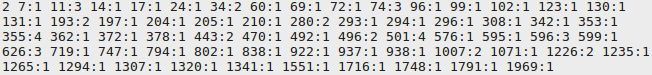
\includegraphics[scale=0.7]{chap5-img/libsvm-example}
	\caption{نمونه‌ای از یک سند منفی در فایل lib-svm}
	\label{chap5-fig1}
\end{figure}


\section{لغت‌نامه‌ی احساس}
\label{chap5sec5}
منظور از لغت‌نامه‌ی احساس یک لغت‌نامه عمومی‌ از پیش ساخته شده است که در آن به ازای هر کلمه برای هر یک از برچسب‌های احساس مثبت، منفی‌ و بی‌طرف وزنی بین ۰ تا ۱ وجود دارد به گونه‌ای که مجموع این مقادیر برای هر کلمه برابر با ۱ است. به عبارت دیگر این لغت‌نامه شامل تعدادی کلمه است که به هیچ دامنه‌ی خاصی‌ وابسته نیستند و برچسب احساسی‌ برای آنها مشخص است. منظور از اینکه این کلمات به هیچ دامنه‌ی خاصی‌ وابسته نیستند و مستقل از دامنه هستند این امر می‌‌باشد که به طور مثال در یک موضوع سینمایی کلمه‌ای مثل ''پیچیده`` برای یک فیلمنامه می‌‌تواند احساسی‌ مثبت به همراه داشته باشد، اما همین کلمه در موضوع علمی‌ بار مثبتی به همراه خود ندارد. از این رو بعضی‌ از کلمات از نظر احساسی‌ وابسته به دامنه‌ای هستند که در آن بحث می‌‌شود و در زمینه‌های مختلف می‌‌توانند بار احساسی‌ متفاوتی داشته باشند. اما لغت‌نامه‌ی احساس از کلماتی ساخته می‌‌شود که در تمام دامنه‌‌ها و زمینه‌ها بار احساسی‌ که به همراه خود دارند ثابت است. به طور مثال کلمه ای‌ مانند
``good''
همیشه یک مفهوم مثبت و کلمه‌ای مانند
``bad'' 
 همه‌‌جا یک مفهوم منفی‌ را می‌‌رسانند.

در بخش‌های بعدی در یکی‌ از آزمایش‌های طراحی شده برای مدل پیشنهادی در این پژوهش از یک لغت‌نامه‌ی احساس به نام
MPQA\footnote{Available at http://mpqa.cs.pitt.edu/}
استفاده می‌‌کنیم. این لغت‌نامه احساسی‌ شامل ۴۰۵۳ کلمه است که در مقابل هر لغت یک بردار ۳تایی‌ وجود دارد که عدد اول نشان دهنده‌ی وزن بی‌طرفی، عدد دوم نشان دهنده‌ی وزن مثبت و عدد سوم نشان دهنده‌ی وزن منفی‌ برای آن لغت است. در مجموع در این لغت‌نامه ۱۵۱۱ کلمه‌ی مثبت و ۲۵۴۲ کلمه‌ی منفی‌ وجود دارد. شکل
\ref{chap5-fig2}
نمونه‌ای از کلمات این لغت‌نامه را نشان می‌‌دهد.
\begin{figure}[!b]
	\centering
	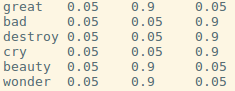
\includegraphics[scale=0.7]{chap5-img/lex-example}
	\caption{نمونه‌ای از لغت‌نامه احساس MPQA شامل ۶ کلمه}
	\label{chap5-fig2}
\end{figure}

\section{جزئیات آموزش مدل پیشنهادی}
\label{chap5sec6}
رويکرد پيشنهادی در اين پژوهش يک مدل احتمالی مولد نظارت شده برای مدل‌سازی همزمان احساس و موضوع در داده‌های متنی می‌باشد که در بخش
\ref{chap4sec5}
به صورت کامل آن را معرفی کردیم. در پایان‌‌نامه برای پياده‌سازی از زبان برنامه‌نويسی پایتون نسخه 2.7 در محيط سيستم عامل لينوکس استفاده شده است. برای پیاده‌سازی ابتدا مدل 
RS
براساس آنچه که در 
\cite{hinton2009replicated}
بيان شده است شبيه‌سازی گرديد، و پس از ارزیابی  و حصول اطمینان از صحت مدل پياده‌سازی شده با بررسی نتايج حاصل از شبيه‌سازی انجام شده با نتايج موجود در 
\cite{hinton2009replicated}
شبيه‌سازی انجام شده را به مدل پيشنهادی در اين پژوهش گسترش داديم.

براساس آنچه که در بخش
\ref{chap5sec4}
بيان کرديم، از پايگاه داده‌ی
MR
در سه حالت مختلف به عنوان داده‌ی ورودی به مدل برای فرآيند آموزش و آزمون استفاده کرديم و نتايج بدست آمده از آزمايشات انجام شده را در بخش‌های بعدی شرح می دهيم. برای آموزش مدل در سه حالات موجود، يعنی با استفاده از ديکشنری های با سايز 2000، 10000 و 24916 ما از الگوريتم 
CD
با مرتبه‌ی ۱ استفاده کرديم. به اين معنی که در مرحله بازسازی داده تنها يک مرحله از اين الگوريتم اجرا شده و جهت گراديان را همان‌طور که آقای 
Hinton
در 
\cite{hinton2002training}
اثبات کرده‌اند تنها با همين يک مرحله تخمين می زنيم. همچنين در هر سه حالت، مدل را به ازای 1000 تکرار\footnote{Epoch, Iteration}
 بر روي کل داده‌هاي آموزش با 
Batch
سايز 1 آموزش داديم و نتايج بدست آمده برای هر حالت را در 2 مرحله، يکی در تکرار ۲۰۰ام و يکی در زمان پايان فرآيند آموزش (تکرار ۱۰۰۰ام) ثبت کرديم. پارامتر ديگری که در آموزش مدل دخيل است تعداد واحدهاي لايه‌ی
Hidden
يا همان تعداد موضوع‌ها است که می توانند متغير باشند. در استفاده از هر 3 ديکشنری، رويکرد پيشنهادی و همچنین مدل 
RS
 را به ازای
$h=\{5,10,15,20,25,30,35,40,45,50,60,70,80,90 \}$
آموزش داديم و نتايج بدست آمده برای حالت‌های مختلف را در ادامه در آزمايش‌های مختلف گزارش می کنيم. برای تمام حالت‌ها از مقدار 
$alfa = 0.001$
برای ضريب يادگيری استفاده کرديم. پارامترهاي 
$W,U,\textbf{a},\textbf{c}$
که به ترتیب وزن بين لايه‌ی 
$Visible$
و
$Hidden$، 
وزن بين لايه‌ی
$Sentiment$
و 
$Hidden$،
باياس لايه‌ی 
$Visible$
و باياس لايه‌ی
$Sentiment$
هستند را با استفاده از مقاديری که به صورت تصادفی از يک توزیع گوسی با ميانگين 0 و واريانس 1 بدست آورديم، مقدار دهی کرديم. همچنين مقدار اوليه‌ی برای باياس لايه‌ی 
$Hidden$
که آن را با 
$\textbf{b}$
نشان داديم را برابر صفر قرار داديم.

\section{مدل‌سازی اسناد و ارزیابی به عنوان یک مدل مولد}
\label{chap5sec7}
در این بخش رویکرد پیشنهادی خودمان را به عنوان یک مدل مولد احتمالاتی با مدل 
RS
در تخمین احتمال برای مشاهده‌ی سندهای پایگاه داده‌های آموزش و تست با استفاده از هر سه لغت‌نامه مورد ارزیابی قرار داده و با تحلیل نتایج بدست آمده نشان می‌‌دهیم که روش پیشنهادی نسبت به روش 
RS
یک روش بهتر در تخمین احتمال برای سندهای دیده نشده و آزمون است. 

برای ارزیابی احتمال محاسبه شده برای مشاهده‌ی اسناد در فرآیند مدل‌سازی مجموعه سند، همان‌طور که در بخش 
\ref{chap5sec1}
گفته شد از یک معیار به نام سرگشتگی استفاده می‌‌شود
\cite{blei2003latent}.
در مباحث مربوط به 
NLP
معیار سرگشتگی پارامتری است که از آن برای مقایسه‌ی مدل‌های احتمالاتی مختلف استفاده می‌شود
\cite{blei2003latent}.
 در فرآیند مدل‌سازی اسناد ما به دنبال تخصیص بالاترین درست‌نمایی به هر سند هستیم و با استفاده از معیار سرگشتگی این مقدار درست‌نمایی 
 محاسبه ‌شده برای هر سند مورد ارزیابی قرار می‌‌گیرد. با توجه به فرمول محاسبه‌ی مقدار سرگشتگی که در رابطه‌ی
\ref{chap5-eq1}
نشان داده شده است می‌‌توان گفت که مقدار این معیار برابر است با معکوس میانگین درست‌نمایی بدست آماده برای هر سند در مقیاس لگاریتمی به ازای تمام کلمات مجموعه اسناد
\cite{blei2003latent}.
 در یک فرآیند مدل‌سازی و با استفاده از یک مدل احتمالی‌ مناسب مقدار سرگشتی باید به صورت پیوسته و یکنوا کاهش یابد و مدلی که مقدار سرگشتگی کمتری بر روی پایگاه داده آزمون داشته باشد در بحث مدل‌سازی اسناد به عنوان مدل بهتری شناخته می‌‌شود
\cite{blei2003latent}.
\begin{align}
	\centering
	\label{chap5-eq1}
	Perplexity = exp\left( - \dfrac{\sum_{n=1}^{N}\log p(\textbf{v}_n)}{\sum_{n=1}^{N}D_n} \right)
\end{align}

در شکل 
\ref{chap5-fig3}
قسمت‌های
\ref{chap5-fig3sub1}
 تا
 \ref{chap5-fig3sub3}
  نمودار تغییرات سرگشتگی در فرآیند آموزش برای مدل پیشنهادی و مدل 
RS
در حالت‌های مخلتف از پایگاه داده‌ی 
MR
نشان داده شده است. همان‌طور که مشاهده می‌‌گردد در هر ۳ نمودار رویکرد پیشنهادی در این پژوهش که یک مدل مشترک احساس موضوع است نسبت به مدل 
RS
که یک رویکرد موضوعی می‌‌باشد با کاهش بهتری در مقدار سرگشتگی همراه است. 

برای رسم نمودارهای شکل
\ref{chap5-fig3}
برای هر دو مدل پیشنهادی و مدل
RS
در هر سه‌ حالت مختلف پایگاه داده، در پایان هر مرحله‌ی آموزش مقدار سرگشتگی با استفاده از رابطه‌ی
\ref{chap5-eq1}
برای تمام پایگاه داده‌ی ‌آموزش محاسبه شده و به ازای هر ۱۰ مرحله از آن میانگین گرفته شده است و در انتها با استفاده از این مقادیر نمودارهای حاصل برای مراحل مختلف آموزش رسم گردیده‌اند.

برای هر سه حالت می‌‌توان مشاهده کرد که مقدار افت سرگشتگی در ابتدای فرایند آموزش نسبت به مراحل پایانی با سرعت بیشتری همراه بوده است، به صورتی‌ که از تکرار ۲۰۰ام تا به انتها مقدار سرگشتی با تغییرات آنچنانی همراه نبوده است. مشاهده‌ی این ویژگی‌ در فرایند آموزش موجب گردید که ما هر دو مدل را برای هر سه حالت مختلف پایگاه داده به ازای دو مقدار ۲۰۰ و ۱۰۰۰ چرخه‌، آموزش داده و از نتایج بدست آماده برای تست مدل بر روی پایگاه داده آزمون استفاده کنیم. 

با دقت در نمودار‌های شکل
\ref{chap5-fig3}
می‌توان نتیجه گرفت که با اضافه کردن و در نظر گرفتن احساس و ساخت یک مدل مشترک احتمالاتی مولد، مانند آنچه که در این پژوهش انجام دادیم، در مرحله‌ی آموزش برای مدل‌سازی اسناد مقدار سرگشتگی با افت بیشتری همراه می‌‌شود و در نتیجه روش احتمالاتی مناسب‌تری برای مدل‌سازی اسناد ساخته می‌‌شود.
	\begin{figure}[!t]
		\centering
		\begin{subfigure}{.45\textwidth}
			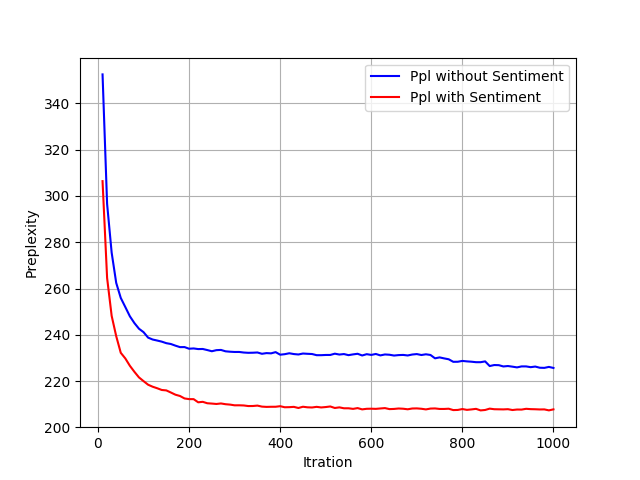
\includegraphics[scale = .4]{chap5-img/ppl_2000}
			\caption{ با استفاده از  لغت‌نامه با اندازه 2000}
			\label{chap5-fig3sub1}
		\end{subfigure}		
		\begin{subfigure}{.45\textwidth}
			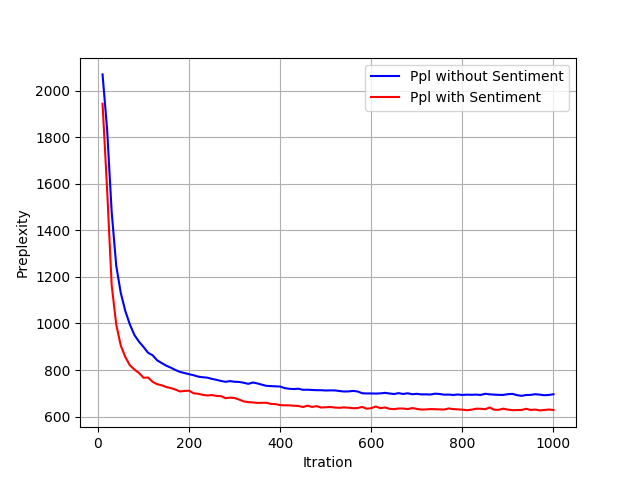
\includegraphics[scale =.4]{chap5-img/ppl_10000}
			\caption{ با استفاده از  لغت‌نامه با اندازه 10000 }
			\label{chap5-fig3sub2}
		\end{subfigure}
		
		\begin{subfigure}{.45\textwidth}
			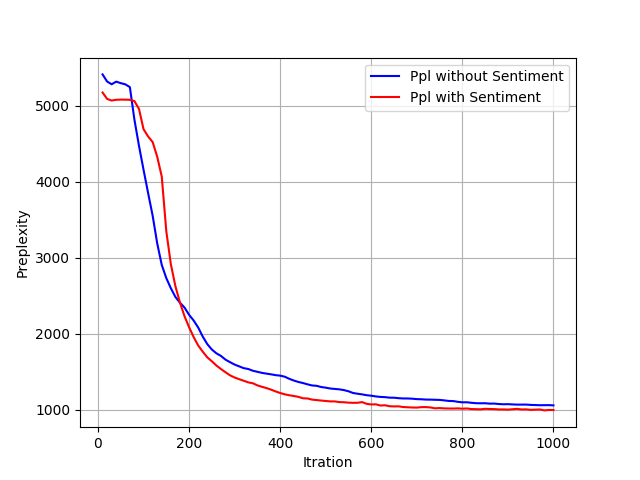
\includegraphics[scale=.4]{chap5-img/ppl_24916}
			\caption{ با استفاده از  لغت‌نامه با اندازه  24916}
			\label{chap5-fig3sub3}
		\end{subfigure}
	\caption{ارزیابی تغییرات سرگشتگی در فرآیند آموزش برروی پایگاه داده‌ی MR  برای مدل پیشنهادی و مدل RS}
	\label{chap5-fig3}
	\end{figure}

مقادير محاسبه شده برای سرگشتگی که در جدول 
\ref{chap5-tb2}
نشان داده شده است نيز دليلی بر اثبات ادعای ما نسبت به بهتر بودن رويکرد پيشنهادی در فرآیند مدل‌سازی به عنوان یک مدل مولد است. در جدول 
\ref{chap5-tb2}
مقدار سرگشتگی برای داده‌هاي تست در پايگاه داده‌ی 
MR
به‌ازای هر 3 ديکشنری مورد استفاده و 2 تکرار 200 و 1000 برای هر کدام محاسبه شده است.

مقادیر بدست آمده برای سرگشتگی در حالت‌های مختلف در جدول
\ref{chap5-tb2}
نشان می‌‌دهد که در حالت‌های استفاده از ۲ لغت‌نامه ۲۰۰۰ و ۱۰۰۰تایی تفاوت مقدار محاسبه شده برای سرگشتگی در مدل هایی که ۱۰۰۰مرحله آموزش دیده‌اند بیشتر است از مدل‌هایی که ۲۰۰ مرحله آموزش دیده‌اند. اما در استفاده از لغت‌نامه‌ی ۲۴۹۱۶تایی شرایط برعکس می‌‌باشد و تفاوت در حالتی که هر دو مدل ۲۰۰ مرحله آموزش دیده‌اند بیشتر از زمانی‌ می‌‌باشد که مدل‌ها ۱۰۰۰ مرحله آموزش دیده‌اند. در اینجا به نمودارهای شکل
\ref{chap5-fig3}
برمی‌‌گردیم و با مقایسه‌ی نمودار
\ref{chap5-fig3sub3}
با نمودارهای
 \ref{chap5-fig3sub1}
و
 \ref{chap5-fig3sub2}
مشاهده می‌کنیم که نمودار مربوط به حالت ۲۴۹۱۶تایی دارای نوسانات بیشتری نسبت به ۲ حالت دیگر می‌‌باشد. به خصوص در  نزدیکی‌ تکرار ۲۰۰ام که مورد بحث ما نیز می‌‌باشد نمودار‌های هر ۲ مدل دچار یک تغییر وضعیت نسبت به یکدیگر گشته و شرایط برای آن‌ها بر عکس شده است.

 با توجه به مقادير بدست آمده برای سرگشتگی برروی پایگاه داده‌ی تست برای مدل پیشنهادی در این پژوهش در مقايسه با مدل 
RS
در جدول 
\ref{chap5-tb2},
مشاهده می‌کنيم که در تمامی حالت‌ها رويکرد پيشنهادی مقدار کمتری را برای سرگشتگی محاسبه کرده است. لذا در تایید آنچه که گفتیم نتيجه گرفته 
می‌شود که راهکار پيشنهادی که با اضافه کردن يک لايه برای احساس نيز همراه است منجر به ساخت يک رويکرد احتمالی مناسب‌ برای مدل‌سازی اسناد 
می‌باشد که در مقایسه با مدل 
RS
نتایج بهتری در بحث مدل‌سازی موضوع بدست می‌دهد.

\begin{table}[!t]
	\centering
	\begin{latin}
	\begin{tabular}{|l|c|c|c|c|}
		\hline
		TestSet Type & Num of Docs & Num of Epoch & Ppl without Sentiment & Ppl with Sentiment \\
		\hline
		MR by 2000 & 1000 & 200 & 400.77 & \textbf{393.69 }\\
		\hline
		MR by 2000 & 1000 & 1000 & 423.89 & \textbf{406.74} \\
		\hline
		MR by 10000 & 1000 & 200 & 1553.52 & \textbf{1529.42} \\
		\hline
		MR by 10000 & 1000 & 1000 & 2028.69 & \textbf{1871.57} \\
		\hline
		MR by 24916 & 1000 & 200 & 4237.65 & \textbf{3898.67}\\
		\hline
		MR by 24916 & 1000 & 1000 & 5842.39 & \textbf{5824.97}\\
		\hline
	\end{tabular}
	\end{latin}
	\caption{تخمین سرگشتگی برای پایگاه داده‌ی Review Movie با استفاده از مدل پیشنهادی}
	\label{chap5-tb2}
\end{table}

\section{مجسم‌سازی موضوع‌ها و ارزیابی دقت در محاسبه‌ی آن‌ها}
\label{chap5sec8}
در بخش
\ref{chap5sec5}
یک لغت‌نامه‌ی احساس به نام
MPQA
معرفی‌ کردیم که شامل ۴۰۵۳ کلمه می‌باشد که برچسب احساس برای آن‌ها مشخص شده است. در این بخش با استفاده از این لغت‌نامه‌ی احساس دقت موضوع‌های یاد گرفته شده توسط مدل را از نظر برچسب احساسی مورد ارزیابی قرار می‌‌دهیم.

با توجه به ساختار رویکرد پیشنهادی که در فصل
\ref{chap5}
توضیح داده شد، می‌‌دانیم که هر یک از واحدهای لایه‌ی
$Hidden$
به تمام واحدها چه در لایه‌ی
$Visible$
و چه در لایه‌ی
$Sentiment$
متصل هستند. هر واحد در لایه‌ی
$Sentiment$
برابر با یک برچسب احساسی‌ و هر واحد در لایه‌ی
$Visible$
متناظر با یک کلمه است. از آنجا که در بحث مدل‌سازی موضوعی اسناد متنی، هر موضوع را به صورت یک توزیع احتمالی چند جمله‌ای بر روی تمام کلمات لغت‌نامه معرفی‌ کردیم لذا می‌دانیم که هر واحد در لایه‌ی
$Hidden$
با یک وزن مشخص به تمام کلمات لغت‌نامه در لایه
$Visible$
متصل است. این وزن  برای هر کلمه نشان دهنده‌ی مقدار اهمیت آن کلمه در آن موضوع است.
\begin{table}[!t]
	\centering
	\begin{latin}
		\begin{tabular}{|c|c|c|c|}
			\hline
			& Total Number & Numb of Positive Words & Num of Negative Words \\ \hline
			NG(2000)  &     155      &          100           &          55           \\ \hline
			RCV(10000) &     950      &          447           &          503          \\ \hline
			MR(24916)  &     3114     &          1242          &         1872          \\ \hline
		\end{tabular}
	\end{latin}
	\caption{فراوانی‌های بدست آمده از مقایسه‌ی کلمات مشترک بین لغت‌نامه‌ی احساسی MPQA با سه لغت‌نامه واژگان}
	\label{chap5-tb3}
\end{table}
ایده‌ی ارزیابی مطرح شده در این بخش از آزمایش‌های انجام شده بر روی مدل‌های معروفی‌ در زمینه‌ی مدل‌سازی موضوعی همچون
DocNADE
و
LDA
گرفته شده است. در مدل
DocNADE
که در بخش 
\ref{chap3sec3sub6}
معرفی گردید و یک روش بر پایه‌ی شبکه عصبی است، برای مجسم‌سازی و نشان دادن موضوع‌های یاد گرفته شده توسط مدل از ماتریس وزن بین لایه‌ی
$Hidden$
و بردار کلمات استفاده می‌‌شود. به این صورت که برای هر موضوع وزن‌های تمام کلمات متصل به آن که در واقع تمام کلمات لغت‌نامه هستند مقایسه شده و بطور مثال ۱۰ کلمه‌ای‌ که دارای بیشترین وزن برای هر موضوع می‌‌باشند به عنوان کلمات متناسب با آن موضوع نشان داده می‌‌شوند. در مدل
LDA
نیز به همین صورت برای نمایش موضوع‌ها عمل می‌‌شود با این تفاوت که در روش
LDA
به جای ماتریس وزن یک ماتریس احتمال داریم و برای هر موضوع بطور مثال ۱۰ کلمه‌ای‌ که بیشترین احتمال در آن موضوع را دارند نشان داده می‌‌شوند.
در این بخش ما نیز از همین ایده کمک گرفته و موضوع‌ها را از نظر برچسب احساسی‌ مورد ارزیابی قرار می‌دهیم.

ابتدا برای هر سه‌ حالت مختلف از پایگاه داده تعداد کلمات مشترک با لغت‌نامه‌ی احساس
MPQA
را محاسبه کردیم. جدول
\ref{chap5-tb3}
نتایج مربوط به این عمل را نشان می‌‌دهد. سپس به ازای هر ۳ حالت از پایگاه داده و ۲ تکرار مختلف برای مرحله‌ی آموزش و همچنین تعداد موضوع‌های مختلف مراحل زیر را به ترتیب انجام دادیم:
\begin{enumerate}
	\item محاسبه‌ی مجموع وزن‌های کلمات مثبت و منفی‌ برای هر موضوع با استفاده از لغت‌نامه‌ی احساس و ماتریس وزن بین لایه‌ی $Visible$ و $Hidden$. 
	\item محاسبه‌ی تفاضل مقادیر حساب شده در مرحله ۱ برای هر موضوع و مرتب کردن مقادیر حاصل به صورت نزولی.
	\item انتخاب ۵ موضوع از ابتدای لیست مرتب (مثبت‌ترین موضوع‌ها) و تخصیص برچسب مثبت به آن‌ها، و ۵ موضوع از انتهای لیست مرتب (منفی‌ترین موضوع‌ها) و تخصیص برچسب منفی‌ به آن‌ها.
	\item مقایسه‌ی برچسب تخصیص داده شده به هر موضوع با وزن‌های متناظر با آن موضوع در اتصال به لایه‌ی
	$Sentiment$
	و محاسبه‌ی دقت.
\end{enumerate}

در مرحله‌ی ۴ام منظور از مقایسه‌ی برچسب تخصیص داده شده به هر موضوع با وزن لایه‌ی
$Sentiment$
به این صورت می‌‌باشد که اگر به یک موضوع در مرحله‌ی ۳ برچسب مثبت اختصاص داده شد، باید وزن متناظر با برچسب احساس مثبت برای آن موضوع در لایه‌ی
$Sentiment$
بیشتر از وزن منفی‌ برای همان موضوع باشد و بر عکس.

نمودار‌های
\ref{chap5-fig4sub1}
و
\ref{chap5-fig4sub2}
نتایج حاصل از این ارزیابی را به ازای ۲۰۰ و ۱۰۰۰ مرحله آموزش نشان می‌‌دهند. همان‌طور که مشاهده می‌‌گردد برای هر ۳ حالت مختلف از پایگاه و تعداد موضوع‌های مختلف تفاوتی‌ بین دقت محاسبه شده برای ۲۰۰ و ۱۰۰۰ مرحله‌‌ی آموزش وجود ندارد. اما با دقت در این نمودارها مشاهده می‌‌گردد که با بزرگ شدن اندازه لغت‌نامه دقت مدل در تخصیص برچسب احساسی‌ به موضوع‌ها نیز افزایش می‌‌یابد.

  مقایسه‌ی اطلاعات موجود در جدول
\ref{chap5-tb3}
برای لغت‌نامه‌های مختلف با نمودار‌های شکل
\ref{chap5-fig4}
علت افزایش دقت به ازای افزایش  اندازه لغت‌نامه را برای ما توجیه می‌‌کند. مشاهده می‌‌شود که با بزرگ شدن اندازه‌ی لغت‌نامه تعداد کلمه‌های مشترک بین آن و لغت‌نامه‌ی احساس نیز افزیش پیدا می‌‌کند و این امر سبب می‌گردد که در فرایند آموزش  موضوع‌های مثبت و منفی‌ بیشتر از یکدیگر تفکیک شده و در نتیجه دقت مدل در یادگیری و تخصیص برچسب احساس به موضوع‌ها افزایش پیدا می‌‌کند.
\begin{figure}[!t]
	\centering
	\begin{subfigure}{.46\textwidth}
		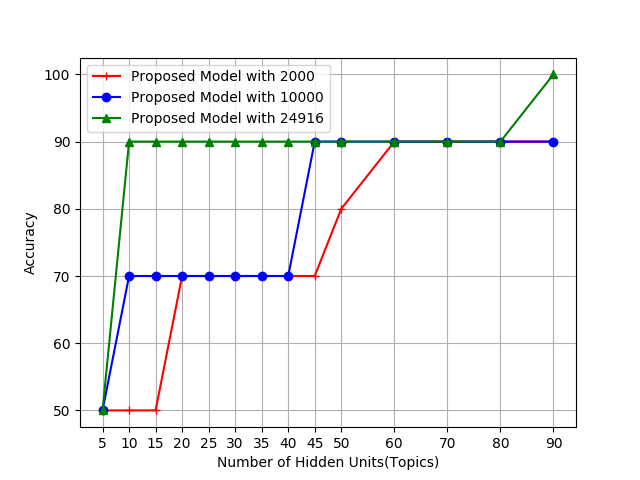
\includegraphics[scale = .48]{chap5-img/v_200}
		\caption{ برای 200 تکرار }
		\label{chap5-fig4sub1}
	\end{subfigure}		
	\begin{subfigure}{.46\textwidth}
		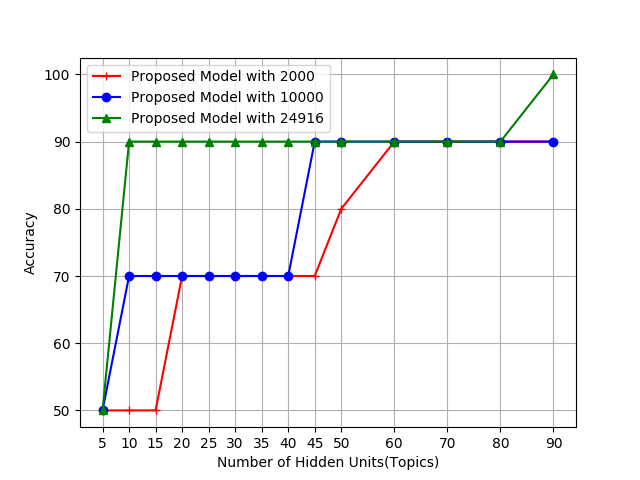
\includegraphics[scale =.48]{chap5-img/v_1000}
		\caption{ برای 1000 تکرار }
		\label{chap5-fig4sub2}
	\end{subfigure}
	\caption{ارزیابی دقت در تخصیص احساس به موضوع‌ها به ۲۰۰ و ۱۰۰۰ مرحله آموزش}
	\label{chap5-fig4}
\end{figure}


\section{طبقه‌بندی احساسی اسناد}
\label{chap5sec9}
در این بخش نتایج حاصل از طبقه‌بندی احساس با استفاده از رویکرد پیشنهادی در این پژوهش را بر روی پایگاه داده‌ی
MR
ارزیابی و گزارش می‌‌کنیم. برای مقایسه‌ی نتایج بدست آمده در بحث طبقه‌بندی احساس با استفاده از مدل پیشنهادی، از یک روش پایه که بر اساس شمارش تعداد کلمات است برای ارزیابی دقت در حالت‌های مختلف بهره می‌‌بریم. همچنین از نتایج بدست آماده برای طبقه‌بندی احساس با استفاده از چند روش معروف نظارت شده مانند ماشین بردار پشتیبان\footnote{Support Vector Machine}
،(SVM)
و دو شبکه عصبی (یک شبکه‌ عصبی با مقادبر اولیه‌ی تصادفی و یک شبکه‌ عصبی با مقادیر اولیه‌ی یادگرفته شده توسط رویکرد پیشنهادی) به منظور ارزیابی پارامترهای یاد گرفته شده توسط مدل استفاده می‌کنیم.

شبکه عصبی‌های استفاده شده در هر دو حالت (مقدار دهی تصادفی و مقدار دهی با پارامترهای یاد گرفته شده توسط مدل پیشنهادی) از دسته شبکه‌های 
MLP\footnote{Multilayer Perceptron}
هستند. در لایه‌ی اول برای هر دو حالت تعداد نورون‌ها برابر با تعداد موضوع‌ها و در لایه‌ی دوم تعداد نورون‌ها برابر با تعداد احساس‌ها هستند. برای هردوی این شبکه‌ها از تابع خطای
Entropy Cross 
استفاده شده است. همچنین در لایه‌ی اول این شبکه‌ها از تابع فعال‌ساز 
tanh
و در لایه‌ی دوم از تابع
Softmax
استفاده شده است.
%
%همچنین علاوه بر یک شبکه عصبی با مقدار دهی‌ اولیه‌ی تصادفی، از یک شبکه عصبی دیگر که مقادیر اولیه در آن با استفاده از پارامترهای یاد گرفته شده توسط مدل پیشنهادی در این پژوهش مقدار دهی‌ می‌‌شوند، برای طبقه‌بندی احساس و ارزیابی نتایج در پایگاه داده‌ی
%MR
%استفاد می‌کنیم که در ادامه نتایج بدست آمده را کامل شرح داده و بررسی‌ می‌‌کنیم.

برای محاسبه‌ی دقت در مدل پایه برای هر سند در پایگاه داده‌ی تست شروع به شمارش کلمات با قطبیت مشخص احساسی‌ می‌‌کنیم. به بیان دیگر برای هر سند تعداد کلمات مثبت و تعداد کلمات منفی را با استفاده از لغت‌نامه‌ی احساس
MPQA
محاسبه می‌کنیم. بعد از محاسبه‌ی تعداد لغات مثبت و منفی‌ برای هر سند اگر این مقدار برای کلمات مثبت در یک سند بیشتر از کلمات منفی‌ بود به سند مورد نظر برچسب مثبت اختصاص دادیم و اگر تعداد کلمات منفی‌ بیشتر بود آن سند را در دسته سندهای منفی‌ دسته‌بندی می‌کنیم.

برای طبقه بندی احساس به کمک رویکرد پیشنهادی در این پژوهش به این صورت عمل می‌کنیم که در ابتد برای هر سند متنی با استفاده از رابطه‌ی
\ref{chap5-eq2}
(این رابطه‌ همان رابطه‌ی \ref{chap4-eq23} است که برای سهولت در اینجا عینا تکرار شده است) مقدار لایه‌ی مخفی متناظر با آن را بدست می آوریم. پس از محاسبه‌ی مقدار لایه‌ی پنهان با استفاده از رابطه‌ی
\ref{chap5-eq2}
مرحله‌ی بعدی محاسبه‌ی لایه‌ی احساس متناظر با سند جاری با استفاده از رابطه‌ی
\ref{chap5-eq3}
(این رابطه‌ نیز همان رابطه‌‌ی \ref{chap4-eq30} است)
است. 
\begin{align}
	\centering
	\label{chap5-eq2}
	p(h_{j}=1|\textbf{V})=\sigma \left( Db_j + \sum_{k=1}^{K}W_{kj}\hat{v}_k \right)
\end{align}
\begin{align}
	\centering
	\label{chap5-eq3}
	p(s_{l}=1|\textbf{h})=\dfrac{exp(c_{l}+\sum_{j=1}^{H}U_{lj}h_j)}{\sum_{l=1}^{S}exp(c_{l}+\sum_{j=1}^{H}U_{lj}h_j)}
\end{align}

همان‌طور که در بخش 
\ref{chap4sec5}
بیان گردید و در رابطه‌ی محاسبه لایه احساس (\ref{chap4-eq30}) مشخص است, چون مقدار این لایه از یک تابع 
$Softmax$
بدست می‌آید لذا به فرم یک توزیع احتمالی است که مجموع درایه‌های آن برابر با 1 است. با بدست آوردن مقدار این لایه‌ی احساس سپس برای تخصیص برچسب به مقادیر این لایه نگاه می‌کنیم و مقدار متناطر با هراحساس که بزرگتر بود برچسب آن سند را برابر با آن احساس انتخاب می کنیم.

نتایج بدست آمده از طبقه‌بندی احساس با استفاده از رویکرد پیشنهادی و مدل پایه برای ۲ حالت مختلف از پایگاه داده‌ در شکل
\ref{chap5-fig5}
نشان داده شده است. برای محاسبه‌ی دقت در طبقه‌بندی احساس با استفاده از مدل پیشنهادی در این پژوهش برای هر ۲ حالت مختلف از پایگاه داده و تعداد موضوع های مختلف از مدل‌هایی که به ازای 1000 تکرار آموزش دیده‌اند استفاده شده است. همچنین برای مقدار دهی اولیه‌ی شبکه عصبی با پارامترهای یاد گرفته شده توسط رویکرد پیشنهادی, از مقادیر بدست آمده برای پارامترها (ماتریس وزن و بایاس) در این حالت (1000 چرخه اموزش) استفاده کردیم.

همانطور که در شکل‌های 
\ref{chap5-fig5sub1}
و
\ref{chap5-fig5sub2}
مشاهده می گردد در هر ۲ حالت دقت طبقه‌بندی برای مدل پیشنهادی با افزایش تعداد موضوع‌ها رو به افزایش بوده است. همچنین در هر ۲ حالت دقت طبقه‌بندی با استفاده از مدل پیشنهادی با افزایش تعداد موضوع‌ها با اختلاف بسيار زیادی از دقت بدست آمده توسط مدل ‌پایه بهتر است. 

%علاوه بر این در حالت استفاده از لغت‌نامه 2000تایی دقت مدل پیشنهادی برای تعداد موضوع های بیشتر از 20 از دقت به دست آمده توسط روش سوم نیز بهتر است. در حالت استفاده لغت‌نامه 2000تایی نیز همچنین برای تعداد موصوع های 80 و 90 دقت به دست آمده توسط مدل پیشنهاد دارای شرایط رقابی با هر 2 مدل شبکه عصبی استفاده شده است, و بااختلاف کمی دیگری پایینتر از انها دارد.  
\begin{figure}[!t]
	\centering
	\begin{subfigure}{.45\textwidth}
		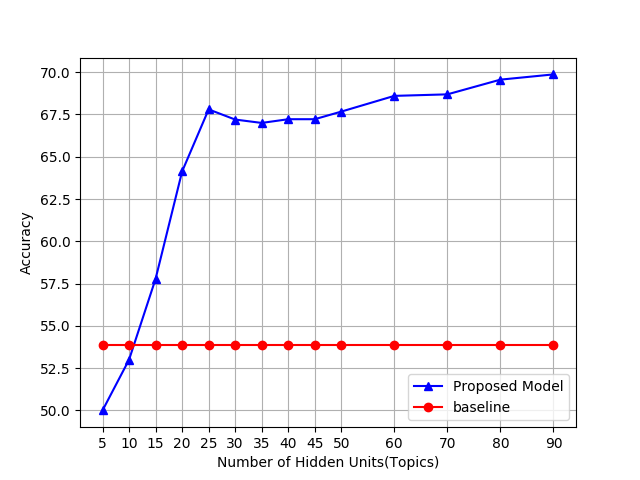
\includegraphics[scale = .4]{chap5-img/sc-a}
		\caption{ با استفاده از  لغت‌نامه با اندازه 2000}
		\label{chap5-fig5sub1}
	\end{subfigure}		
	\begin{subfigure}{.45\textwidth}
		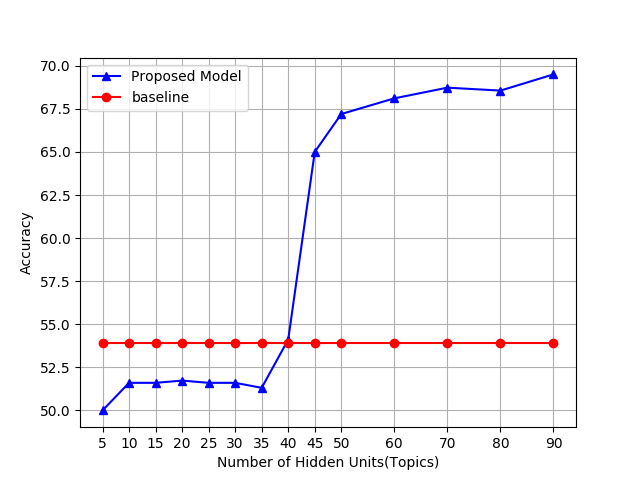
\includegraphics[scale =.4]{chap5-img/sc-b}
		\caption{ با استفاده از  لغت‌نامه با اندازه 10000 }
		\label{chap5-fig5sub2}
	\end{subfigure}
	\caption{طبقه‌بندی احساس در پایگاه داده‌ی MR با استفاده از مدل پیشنهادی و مدل پایه برای موضوع‌های مختلف }
	\label{chap5-fig5}
\end{figure}

با مقایسه‌ي دقت بدست آمده برای طبقه‌بندی احساس به کمک رویکرد پیشنهادی و با استفاده از لغت‌نامه 10000تایی (شکل \ref{chap5-fig5sub2}) با نمودار شکل 
\ref{chap5-fig4sub2}
نتایج جالبی بدست می آید. در نمودار شکل 
\ref{chap5-fig5sub2}
دقت طبقه‌بندی احساس برای روش پیشنهادی در بازه‌ی تعداد موضوع های 40 تا 45 دچار یک جهش بزرگ و افزایش دقت با شیب زیادی می شود. با مقایسه این جهش و بررسی عمیق‌تر نمودار شکل 
\ref{chap5-fig4sub2}
مشاهده می‌شود که ارزیابی دقت در تخصیص برچسب احساس به موضوع‌ها برای لغت‌نامه 10000تایی در بازه 40 تا 45 موضوع با یک افزایش با شیب بسيار زیاد همراه است. لذا نتیجه می شود که هرچه دقت در تخصیص برچسب احساس به موضوع‌ها بالاتر رود, یا به عبارت دیگر هرچه موضوع‌های متمایزتری از نظر احساسی داشته باشیم دقت در بحث طبقه‌بندی احساس نیز بالاتر می‌رود.

شکل 
\ref{chap5-fig6}
دقت نتایج حاصل از طبقه‌بندی احساس با استفاده از ۳ مدل مختلف را نشان می‌دهد. با دقت در نمودارهای شکل
\ref{chap5-fig6}
مشاهده می‌شود که در هر دو حالت مورد نظر برای پایگاه داده, دقت بدست آمده با استفاده از شبکه عصبی با مقدار دهی اولیه توسط پارامترهای یاد گرفته شده در روش پیشنهادی, از دقت بدست آمده توسط هر دو روش دیگر بهتر است.

در حالت استفاده از لغت‌نامه 10000تایی همان‌طور که در شکل 
\ref{chap5-fig6sub2}
مشخص است, تنها زمانی که تعداد موضوع‌ها برابر با 20 و 70 هستند دقت هر دو شبکه عصبی با هم برابر است. در سایر موارد شبکه با مقدار دهی
 اولیه‌ی پارامترها نسبت به هر 3 مدل دیگر نتایج بهتری داشته است. به طور کلی نتیجه می‌شود که در فرآیند طبقه‌بندی احساس، شبکه‌ی عصبی که مقادیر آن توسط پارامترهای یاد گرفته شده توسط مدل پیشنهادی مقدار دهی اولیه می‌شوند از عملکرد بهتری نسبت به سایر مدل‌ها برخوردار است.
\begin{figure}[!t]
	\centering
	\begin{subfigure}{.45\textwidth}
		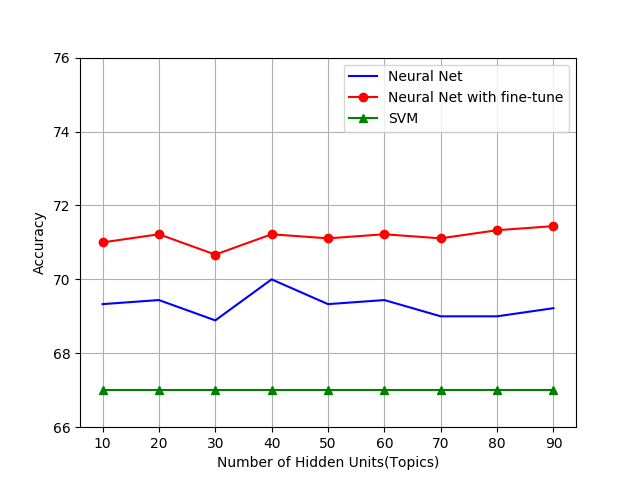
\includegraphics[scale = .4]{chap5-img/sc-c}
		\caption{ با استفاده از  لغت‌نامه با اندازه 2000}
		\label{chap5-fig6sub1}
	\end{subfigure}		
	\begin{subfigure}{.45\textwidth}
		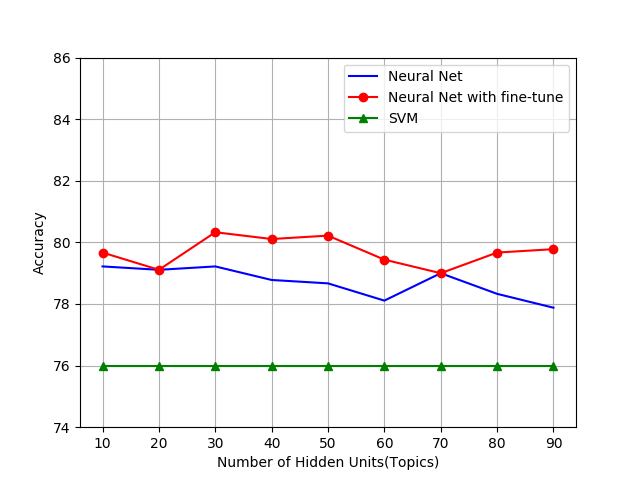
\includegraphics[scale =.4]{chap5-img/sc-d}
		\caption{ با استفاده از  لغت‌نامه با اندازه 10000 }
		\label{chap5-fig6sub2}
	\end{subfigure}
	\caption{طبقه‌بندی احساس در پایگاه داده‌ی MR با استفاده از مدل‌های شبکه عصبی با مقدار دهی اولیه برای وزن‌ها و بایاس‌ها، شبکه عصبی و SVM }
	\label{chap5-fig6}
\end{figure}

\section{بازیابی اطلاعات}
\label{chap5sec10}
با توجه به اینکه رویکرد پیشنهادی در  این پژوهش یک روش مولد برای مدل‌سازی همزمان احساس و موضوع است، لذا گام نخست برای ارزیابی این مدل در بحث بازیابی اطلاعات استفاده از پایگاه داده‌ای است که علاوه بر برچسب احساس برای اسناد، دارای برچسب موضوع برای هر سند نیز باشد. با توجه به عدم وجود یک چنین پایگاه داده‌ای، در این پژوهش ۲ پایگاه داده که همزمان شامل برچسب احساس و برچسب موضوع هستند ساخته شده است.

اولین پایگاه داده‌ی احساس‌-موضوع ساخته شده در این قسمت با تخصیص برچسب احساس به دیتاست
20NG
ساخته می‌‌شود. در بخش
\ref{chap5sec11}
پایگاه داده‌ی
20NG
را معرفی‌ کردیم. همان‌طور که بیان شد
20NG
یک پایگاه داده‌ی معیار در بخش مدل‌سازی موضوعی است. اسناد موجود در
20NG
شامل ۲۰ گروه مختلف می‌‌شوند که هر یک از گروه‌ها در مورد یک موضوع خاص، مانند سیاسی، ورزشی، علمی‌ و غیره هستند. برای اضافه کردن احساس به این مجموعه، مانند آنچه که در بخش
\ref{chap5sec9}
برای بدست آوردن دقت مدل پایه برای طبقه‌بندی احساس گفته شد، برای هر سند به شمارش تعداد کلمات با قطبیت مشخص احساسی‌ با استفاده از 
لغت‌نامه‌ی احساس
MPQA
کردیم. سپس برای هر سند اگر تعداد کلمات مثبت بیشتر بود به آن سند برچسب مثبت اختصاص دادیم و برعکس. در فایل
lib-svm
که برای این پایگاه داده ساخته می‌‌شود، برای هر سند عدد اول نشان دهنده‌ی احساس (۱ مثبت، ۲ منفی‌) و عدد دوم (عددی از ۱ تا ۲۰) نشان 
دهند‌ه‌ی موضوع مانند:\\ 
\begin{latin}
	SentimentLabel \ TopicLabel \ <ID:Count> \ <ID:Count> \ <ID:Count> \ ... 
\end{latin} 
برای آن سند است.

پایگاه داده‌ی دومی‌ که برای ارزیابی رویکرد پیشنهادی در این پژوهش در بحث بازیابی اطلاعات ساخته می‌‌شود، از ترکیب چند دیتاست بدست می‌‌آید. 
پایگاه داده‌های
MR
و
MDS
در بخش‌های
\ref{chap5sec3}
و
\ref{chap5sec12}
به ترتیب معرفی‌ شدند. هر کدام از این ۵ پایگاه داده 
(
MDS
 شامل ۴ بخش مختلف با ۲۰۰۰ سند در هر بخش است) 
تنها شامل برچسب احساس هستند. می‌‌توان هر کدام از این مجموعه اسناد را به صورت یک موضوع خاص در نظر گرفت. به عبارت دیگر با کنار هم قرار دادن این پایگاه داده‌ها می‌‌توان یک پایگاه داده بزرگتر ایجاد کرد. این دیتاست جدید ساخته شده شامل ۱۰۰۰۰ سند است که ۵۰۰۰تا از آن‌ها دارای برچسب مثبت و ۵۰۰۰تای دیگر دارای برچسب منفی‌ هستند. همچنین این پایگاه داده‌ی جدید شامل ۵ موضوع مختلف که بازبینی‌ فیلم، کتاب، دی‌وی‌دی، وسایل آشپزخانه و وسایل الکترونیکی‌ هستند،می‌‌شود. پس اتمام مرحله‌ی پیش‌پردازش هر کدام از این اسناد با استفاده از لغت‌نامه پایگاه داد‌ه‌ی
20NG
(۲۰۰۰ کلمه) به فایل
libsvm
تبدیل شدند. از ۱۰۰۰۰ سند نتیجه که با ترکیب این ۵ پایگاه داده بدست می‌‌آید، ۷۵۰۰ سند برای مجموعه آموزش با توزیع مساوی از نظر برچسب احساس (۳۷۵۰ سند مثبت و ۳۷۵۰ سند منفی‌) و موضوع ( ۱۵۰۰ سند از هر موضوع که ۷۵۰تای آن مثبت و ۷۵۰تای دیگر منفی‌ هستند) انتخاب شدند و مابقی 
مجموعه‌ی تست را که شامل ۲۵۰۰ سند (۵۰۰ سند از هر موضوع که ۲۵۰تای آن مثبت و ۲۵۰تای آن منفی‌ هستند) است، تشکیل می‌‌دهند. این پایگاه داده‌ی ساخته شده را به اختصار 
MRMDS
نام‌گذاری می‌کنیم.

\begin{figure}[!b]
	\centering
	\begin{subfigure}{.45\textwidth}
		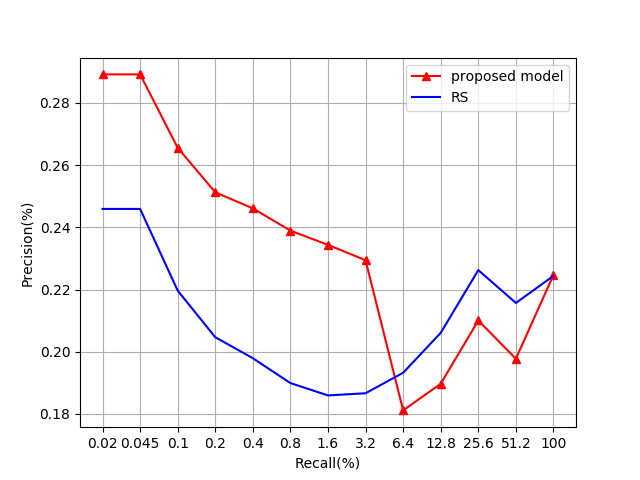
\includegraphics[scale = .4]{chap5-img/ir-1}
		\caption{پایگاه داده‌ی Groups News 20}
		\label{chap5-fig7sub1}
	\end{subfigure}		
	\begin{subfigure}{.45\textwidth}
		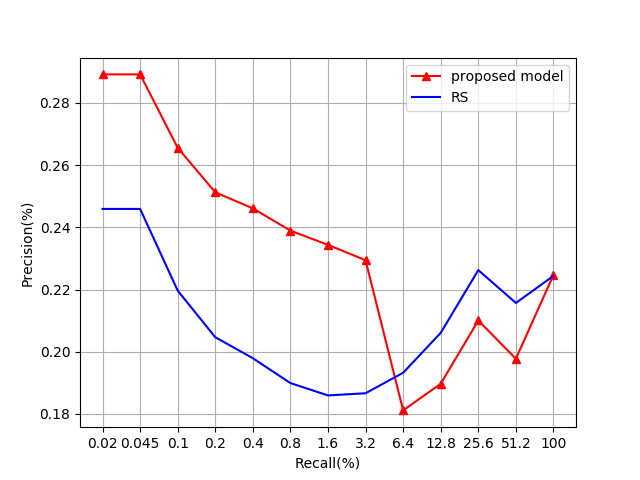
\includegraphics[scale =.4]{chap5-img/ir-2}
		\caption{ پایکاه داده‌ی MRMDS}
		\label{chap5-fig7sub2}
	\end{subfigure}
	\caption{بازیابی اطلاعات با استفاده ۲ پایگاه داده‌ی Groups News 20 و MRMDS برای رویکرد پیشنهادی و مدل RS}
	\label{chap5-fig7}
\end{figure}
پس از ساخت پایگاه داده‌های مورد نیاز، به ارزیابی بازیابی اطلاعات برای رویکرد پیشنهادی در این پژوهش در مقایسه با مدل
RS
که در بخش
\ref{chap3sec3sub5}
معرفی‌ شد می‌‌پردازیم. هدف از این ارزیابی مشاهده تاثیر در نظر گرفتن احساس برای بازیابی اطلاعات با استفاده از ساختار پیشنهادی در این پژوهش است. برای ارزیابی مورد نظر از نمودار صحت در برابر بازیابی\footnote{Precision vs Recall}
استفاده می‌‌کنیم. این نمودار به عنوان معروف‌ترین معیار در بحث ارزیابی بازیابی اطلاعات و مقایسه‌ی روش‌های مختلف در این زمینه شناخته می‌‌شود. برای رسم این نمودار از مقادیر مختلف صحت و بازیابی که توسط هر مدل بدست می‌‌آیند در برابر یکدیگر استفاده می‌‌شود. روابط
\ref{chap5-eq4}
و
\ref{chap5-eq5}
شیوه‌ی محاسبه‌ی مقادیر بازیابی و صحت را نشان می‌‌دهند. منظور از
TP
در هر دو رابطه‌ی
\ref{chap5-eq4}
و
\ref{chap5-eq5}
مثبت‌های واقعی‌\footnote{True Positive}
 است که آن را برابر با تعداد اسنادی تعریف می‌‌کنیم که برچسب موضوعی برای آن‌ها همان برچسب مورد نظر ما است و مدل نیز آن‌ها را 
درست تشخیص داده است.
$C^+$
در رابطه‌ی
\ref{chap5-eq4}
نشان دهنده‌ی تعداد کل سندهای موجود با برچسب مورد نظر ما در پایگاه داده است و
$R^+$
نشان دهنده‌ی تعداد اسنادی است که مدل آن‌ها را برای ما هماهنگ با برچسب مورد نظر ما تشخیص داده است.
\begin{align}
	\centering
	\label{chap5-eq4}
	recall = \dfrac{TP}{C^+}
\end{align}
\begin{align}
	\centering
	\label{chap5-eq5}
	precision = \dfrac{TP}{R^+}
\end{align}
نمودار‌های شکل
\ref{chap5-fig5}
نتایج حاصل از ارزیابی بازیابی اطلاعات برای رویکرد پیشنهادی در این پژوهش و همچنین مدل
RS
را نشان می‌‌دهند. همان‌طور که مشاهده می‌‌شود برای هر ۲ نمودار شکل
\ref{chap5-fig5}
بخصوص نمودار
\ref{chap5-fig5sub1}
روش پیشنهادی در این پژوهش عملکرد بهتری را در مقایسه با مدل
RS
در بحث بازیابی اطلاعات داشته است. برای محاسبه مقادیر صحت و بازیابی و رسم نمودار‌های شکل
\ref{chap5-fig5}
به این صورت عمل شده است که، ابتدا بر روی هر کدام از پایگاه داده‌ها مدل پیشنهادی در این پژوهش بدون در نظر گرفتن برچسب موضوع و تنها با برچسب احساس و لایه‌ی مخفی با اندازه 50، و همچنین روش
RS
بدون در نظر گرفتن برچسب‌های احساس و موضوع و لابه‌ی مخفی با اندازه 50 به ازای ۵۰۰ تکرار آموزش داده شده‌اند. در مرحله‌ی بعدی برای تک‌تک سند‌های مجموعه‌ی تست در هر پایگاه داده مقدار شباهت کسینوسی\footnote{Cosine Similarity}
هر سند با تمام اسناد پایگاه داده‌ی آموزش محاسبه شده و مقادیر دقت و بازیابی به دست آمده‌اند. در ادامه مقادیر بدست آمده برای صحت برای کل پایگاه داده‌ی تست میانگین گرفته می‌‌شوند و نمودار‌های
\ref{chap5-fig5sub1}
و
\ref{chap5-fig5sub2}
رسم می‌‌شوند.

\section{نتیجه‌گیری}
در این فصل رویکرد پیشنهادی در این پژوهش که یک مدل مولد احتمالاتی نظارت شده برای مدل‌سازی مشترک موضوع و احساس در داده‌های متنی است مورد ارزیابی‌های مختلفی‌ قرار گرفت.  برای انجام این ارزیابی‌ها از چند پایگاه داده معروف در بحث مدل‌سازی موضوع و احساس استفاده گردید که هر کدام از آن‌ها در بخش‌های متفاوتی معرفی‌ و به تفصیل شرح داده شدند. همچنین در این فصل یک لغت‌نامه‌ی احساس معرفی‌ شد و با ساختار آن آشنا شدیم. در فصل بعدی نتجه‌گیری نهایی از پژوهش و پیشنهادات آینده مطرح می‌گردند.
